
%(BEGIN_QUESTION)
% Copyright 2006, Tony R. Kuphaldt, released under the Creative Commons Attribution License (v 1.0)
% This means you may do almost anything with this work of mine, so long as you give me proper credit

%Determine the voltmeter's indication in this thermocouple circuit (type E) for the following temperatures:

Finn ut hva voltmeteret vil vise i denne kretsen med termoelement av type E, for følgende temperaturer

$$\includegraphics[width=15.5cm]{i00381x01.eps}$$

\begin{itemize}
\item{$\bullet$} $T_{measurement}$ = 1500$^{o}$ C ; $T_{reference}$ = 65$^{o}$ C ; Voltmeter voltage = ??? 
\item{$\bullet$} $T_{measurement}$ = 212$^{o}$ C ; $T_{reference}$ = 74$^{o}$ C ; Voltmeter voltage = ??? 
\item{$\bullet$} $T_{measurement}$ = -360$^{o}$ C ; $T_{reference}$ = 32$^{o}$ C ; Voltmeter voltage = ??? 
\item{$\bullet$} $T_{measurement}$ = -132$^{o}$ C ; $T_{reference}$ = -30$^{o}$ C ; Voltmeter voltage = ??? 
\medskip

\underbar{file i00381no}
%(END_QUESTION)





%(BEGIN_ANSWER)

\begin{itemize}
\item{$\bullet$} $T_{measurement}$ = 1500$^{o}$ F ; $T_{reference}$ = 65$^{o}$ F ; Voltmeter voltage = 61.145 mV 
\item{$\bullet$} $T_{measurement}$ = 212$^{o}$ F ; $T_{reference}$ = 74$^{o}$ F ; Voltmeter voltage = 4.925 mV 
\item{$\bullet$} $T_{measurement}$ = -360$^{o}$ F ; $T_{reference}$ = 32$^{o}$ F ; Voltmeter voltage = -9.229 mV 
\item{$\bullet$} $T_{measurement}$ = -132$^{o}$ F ; $T_{reference}$ = -30$^{o}$ F ; Voltmeter voltage = -2.876 mV 
\medskip

%(END_ANSWER)





%(BEGIN_NOTES)


%INDEX% Measurement, temperature: thermocouple

%(END_NOTES)


